\documentclass[10pt,a4paper]{article}

\usepackage[utf8]{inputenc}
\usepackage[T1]{fontenc}
\usepackage[left=2.25cm,right=2.25cm,top=2.1cm,bottom=2.2cm]{geometry}
\usepackage{array}
\usepackage{enumitem}
\usepackage{graphicx}
\usepackage{xcolor}
\usepackage{titlesec}
\usepackage{fancyhdr}
\usepackage[most]{tcolorbox}
\usepackage{hyperref}
\usepackage{booktabs}
\usepackage{float}

\renewcommand{\contentsname}{Índice}
\renewcommand{\figurename}{Figura}
\renewcommand{\tablename}{Tabla}
\renewcommand{\refname}{Bibliografía}

\definecolor{negro}{RGB}{0,0,0}
\definecolor{gris}{RGB}{90,90,90}
\definecolor{grisclaro}{RGB}{150,150,150}

\hypersetup{
  colorlinks=true,
  linkcolor=negro,
  urlcolor=negro,
  citecolor=negro,
  hypertexnames=false,
  pdftitle={Evaluación Sumativa 1 - Framingham},
  pdfauthor={Alexander Sepúlveda Ormazábal}
}

\titleformat{\section}{\large\bfseries\color{negro}}{\thesection.}{0.5em}{}
\titleformat{\subsection}{\normalsize\bfseries\color{negro}}{\thesubsection}{0.5em}{}
\titlespacing*{\section}{0pt}{1.0em}{0.25em}
\titlespacing*{\subsection}{0pt}{0.65em}{0.2em}

\pagestyle{fancy}
\fancyhf{}
\fancyfoot[L]{\footnotesize\color{gris}Magíster en Ciencia de Datos e Inteligencia Artificial}
\fancyfoot[R]{\footnotesize\color{gris}\thepage}
\renewcommand{\headrulewidth}{0pt}
\renewcommand{\footrulewidth}{0.4pt}
\setlength{\headheight}{13pt}

\newtcolorbox{infobox}[1][Información de la evaluación]{
  colback=black!3,colframe=negro,fonttitle=\bfseries,coltitle=white,title={#1},
  boxrule=0.6pt,arc=1pt,left=8pt,right=8pt,top=5pt,bottom=5pt,breakable
}

\newcommand{\proyTitulo}{Análisis estadístico del riesgo de enfermedad coronaria a diez años}
\newcommand{\proyIntegrantes}{Alexander Sepúlveda Ormazábal}
\newcommand{\proyDataset}{Framingham Heart Study}
\newcommand{\proyDocente}{Jean Paul Maidana González}
\newcommand{\proyFecha}{14/10/2026}
\newcommand{\proyRepo}{\url{https://github.com/alexander-seor/MCDI501-Proyecto-Framingham}}

\setlength{\parindent}{0pt}
\setlength{\parskip}{0.28em}
\setlength{\emergencystretch}{2em}
\setlist[itemize]{leftmargin=1.35em,itemsep=0.1em,topsep=0.15em}
\setlist[enumerate]{leftmargin=1.55em,itemsep=0.1em,topsep=0.15em}

\begin{document}
\pagenumbering{gobble}

\thispagestyle{empty}
\begin{center}
\vspace*{0.5cm}

\includegraphics[height=4.1cm]{logo_unab.png}\\[0.9cm]

{\footnotesize\color{gris}\MakeUppercase{Magíster en Ciencia de Datos e Inteligencia Artificial}}\\[0.12cm]
{\footnotesize\color{grisclaro}MCDI501: Estadística Computacional para la Toma de Decisiones}\\[1.45cm]

{\Large\bfseries\color{negro}Evaluación Sumativa 1}\\[0.35cm]
{\large\color{negro}Análisis Exploratorio e Inferencial}\\[0.75cm]
{\small\itshape\color{gris}Informe técnico individual \textperiodcentered\ 20\,\%}
\end{center}

\vspace{1.1cm}

\begin{flushleft}
\newcommand{\datodeportada}[2]{%
  \noindent
  \begin{minipage}[t]{4.0cm}\vspace{0pt}\bfseries\color{negro}#1\end{minipage}%
  \hspace{0.45cm}%
  \begin{minipage}[t]{10.6cm}\vspace{0pt}#2\end{minipage}%
  \par\vspace{0.45em}%
}
\datodeportada{Título del proyecto:}{\proyTitulo}
\datodeportada{Estudiante:}{\proyIntegrantes}
\datodeportada{Dataset:}{\proyDataset}
\datodeportada{Docente:}{\proyDocente}
\datodeportada{Fecha:}{\proyFecha}
\datodeportada{Repositorio GitHub:}{\proyRepo}
\end{flushleft}

\clearpage
\pagenumbering{arabic}

\begin{infobox}
\textbf{Fase del proyecto:} Fase 2: Búsqueda y recopilación de información\\
\textbf{Modalidad:} Individual\qquad\textbf{Ponderación:} 20\,\% de la nota final\\
\textbf{Entregables:} Informe PDF (máx. 8 páginas, sin anexos) \textperiodcentered\ Notebook \texttt{.ipynb} \textperiodcentered\ Repositorio GitHub\\
\textbf{Resultado de aprendizaje (RA1):} aplicar probabilidad e inferencia estadística en problemas de decisión bajo incertidumbre.\\
\textbf{Indicadores:} ID1.2, ID1.3 e ID1.4.
\end{infobox}

\vspace{0.35em}
\tableofcontents
\newpage

% Guía oficial: carga, estructura, tipos, faltantes, duplicados, inconsistencias y limpieza básica.
\section{Preparación y carga de datos}

El proyecto estudia factores demográficos, conductuales y clínicos asociados con la ocurrencia de enfermedad coronaria durante diez años. Se utiliza una versión del \textit{Framingham Heart Study} publicada en Kaggle \cite{dileep}, con 4.238 personas y 16 variables. La respuesta \texttt{TenYearCHD} toma el valor 1 cuando se registra el evento y 0 en caso contrario. La pregunta de análisis es: \textit{¿qué diferencias se observan entre quienes desarrollaron y quienes no desarrollaron enfermedad coronaria durante el seguimiento?}

El archivo \texttt{framingham.csv} se cargó en Python sin modificarlo. Se verificaron dimensiones, tipos computacionales, valores únicos, rangos, duplicados y codificaciones. No se encontraron filas duplicadas ni valores fuera de las categorías o rangos admisibles. La Tabla~\ref{tab:calidad} resume la ausencia de datos. Cada análisis utiliza casos disponibles e informa su tamaño muestral; no se imputaron valores en esta fase para evitar introducir supuestos no evaluados.

\begin{table}[H]
\centering
\caption{Variables con datos faltantes.}
\label{tab:calidad}
\small
\begin{tabular}{lrr@{\hspace{1.2cm}}lrr}
\toprule
\textbf{Variable} & \textbf{Faltantes} & \textbf{\%} & \textbf{Variable} & \textbf{Faltantes} & \textbf{\%} \\
\midrule
\texttt{education} & 105 & 2,48 & \texttt{totChol} & 50 & 1,18 \\
\texttt{cigsPerDay} & 29 & 0,68 & \texttt{BMI} & 19 & 0,45 \\
\texttt{BPMeds} & 53 & 1,25 & \texttt{heartRate} & 1 & 0,02 \\
\texttt{glucose} & 388 & 9,16 & & & \\
\bottomrule
\end{tabular}
\end{table}

Las variables binarias se trataron como cualitativas nominales; \texttt{education}, como ordinal; \texttt{age} y \texttt{cigsPerDay}, como cuantitativas discretas; y las mediciones clínicas restantes, como cuantitativas continuas. Esta distinción evita interpretar como promedios los códigos 0/1 y orienta la elección de tablas, gráficos y pruebas.

% Guía oficial: descriptiva, visualizaciones, correlaciones y análisis bivariado contextualizado.
\section{Análisis exploratorio de datos}

\subsection{Estadística descriptiva}

La Tabla~\ref{tab:descriptiva} combina medidas de tendencia central y dispersión. Cigarrillos diarios y glucosa presentan asimetría positiva; por ello, su media se interpreta junto con la mediana y el rango intercuartílico (RIC). La presión sistólica y el colesterol también exhiben observaciones elevadas.

\begin{table}[H]
\centering
\caption{Resumen de variables numéricas.}
\label{tab:descriptiva}
\small
\begin{tabular}{lrrrrr}
\toprule
\textbf{Variable} & \textbf{$n$} & \textbf{Media} & \textbf{Mediana} & \textbf{DE} & \textbf{RIC} \\
\midrule
Edad (años) & 4.238 & 49,58 & 49,00 & 8,57 & 14,00 \\
Cigarrillos/día & 4.209 & 9,00 & 0,00 & 11,92 & 20,00 \\
Colesterol (mg/dL) & 4.188 & 236,72 & 234,00 & 44,59 & 57,00 \\
Presión sistólica (mmHg) & 4.238 & 132,35 & 128,00 & 22,04 & 27,00 \\
Presión diastólica (mmHg) & 4.238 & 82,89 & 82,00 & 11,91 & 14,88 \\
IMC & 4.219 & 25,80 & 25,40 & 4,08 & 4,97 \\
Frecuencia cardíaca (lpm) & 4.237 & 75,88 & 75,00 & 12,03 & 15,00 \\
Glucosa (mg/dL) & 3.850 & 81,97 & 78,00 & 23,96 & 16,00 \\
\bottomrule
\end{tabular}
\end{table}

La respuesta está desbalanceada: 644 personas desarrollaron enfermedad coronaria (15,20\,\%) y 3.594 no la desarrollaron (84,80\,\%). El 31,05\,\% presenta antecedente de hipertensión, 49,41\,\% registra tabaquismo actual y 2,57\,\% tiene diabetes. La Figura~\ref{fig:objetivo} muestra simultáneamente el desbalance y la calidad de información.

\begin{figure}[H]
\centering
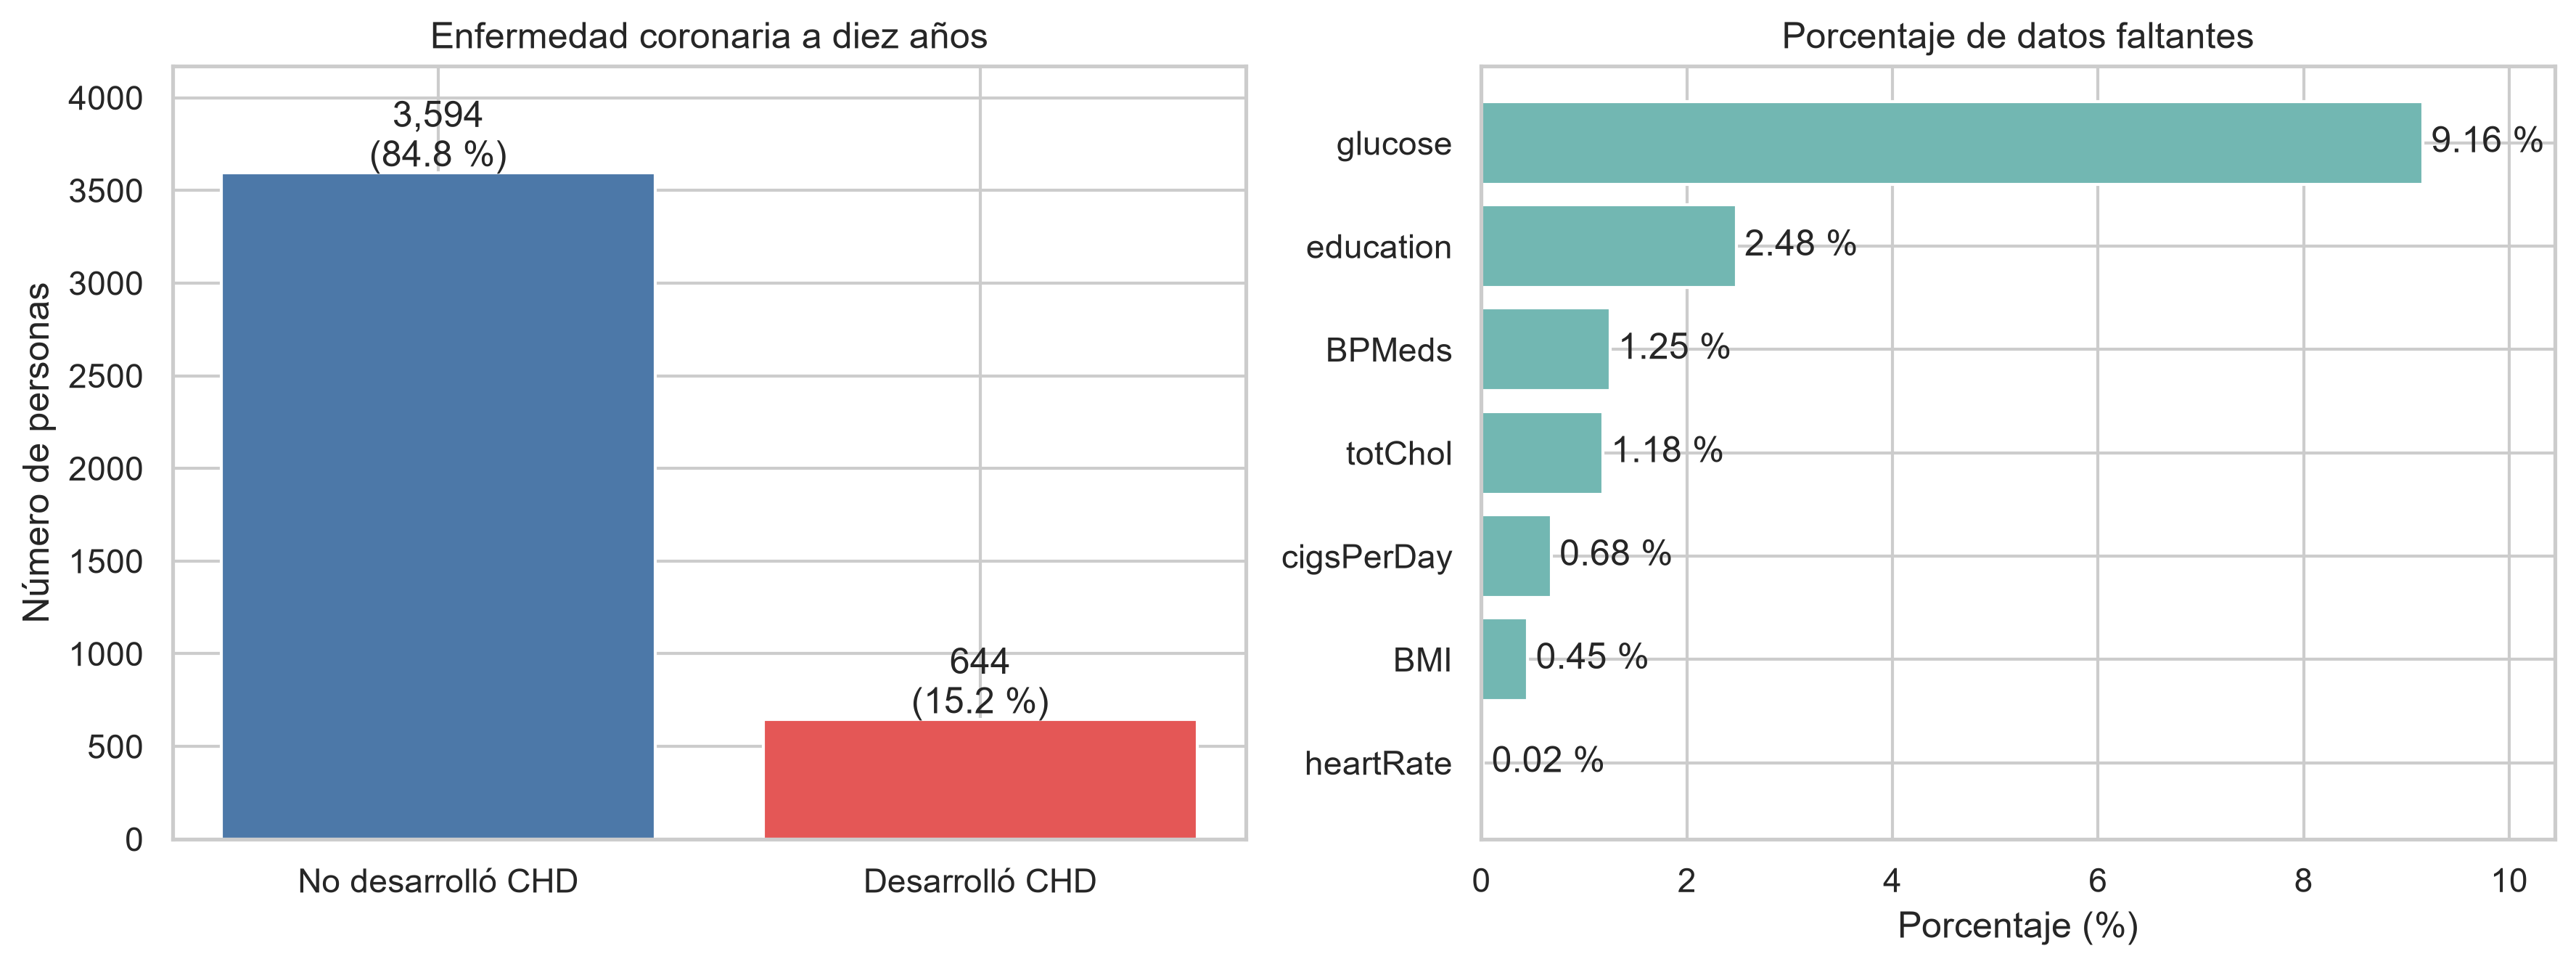
\includegraphics[width=0.86\textwidth]{../figuras/figura_1_objetivo_faltantes.png}
\caption{Distribución de la respuesta y porcentaje de datos faltantes.}
\label{fig:objetivo}
\end{figure}

\subsection{Relaciones bivariadas}

La matriz de Pearson de la Figura~\ref{fig:correlaciones} identifica relaciones lineales. Presión sistólica y diastólica presentan la asociación más alta ($r=0,78$). Respecto de \texttt{TenYearCHD}, las correlaciones mayores corresponden a edad ($r=0,23$) y presión sistólica ($r=0,22$). Debido a que la respuesta es binaria, estos valores equivalen a correlaciones punto-biseriales; no implican causalidad y pueden omitir relaciones no lineales.

\begin{figure}[H]
\centering
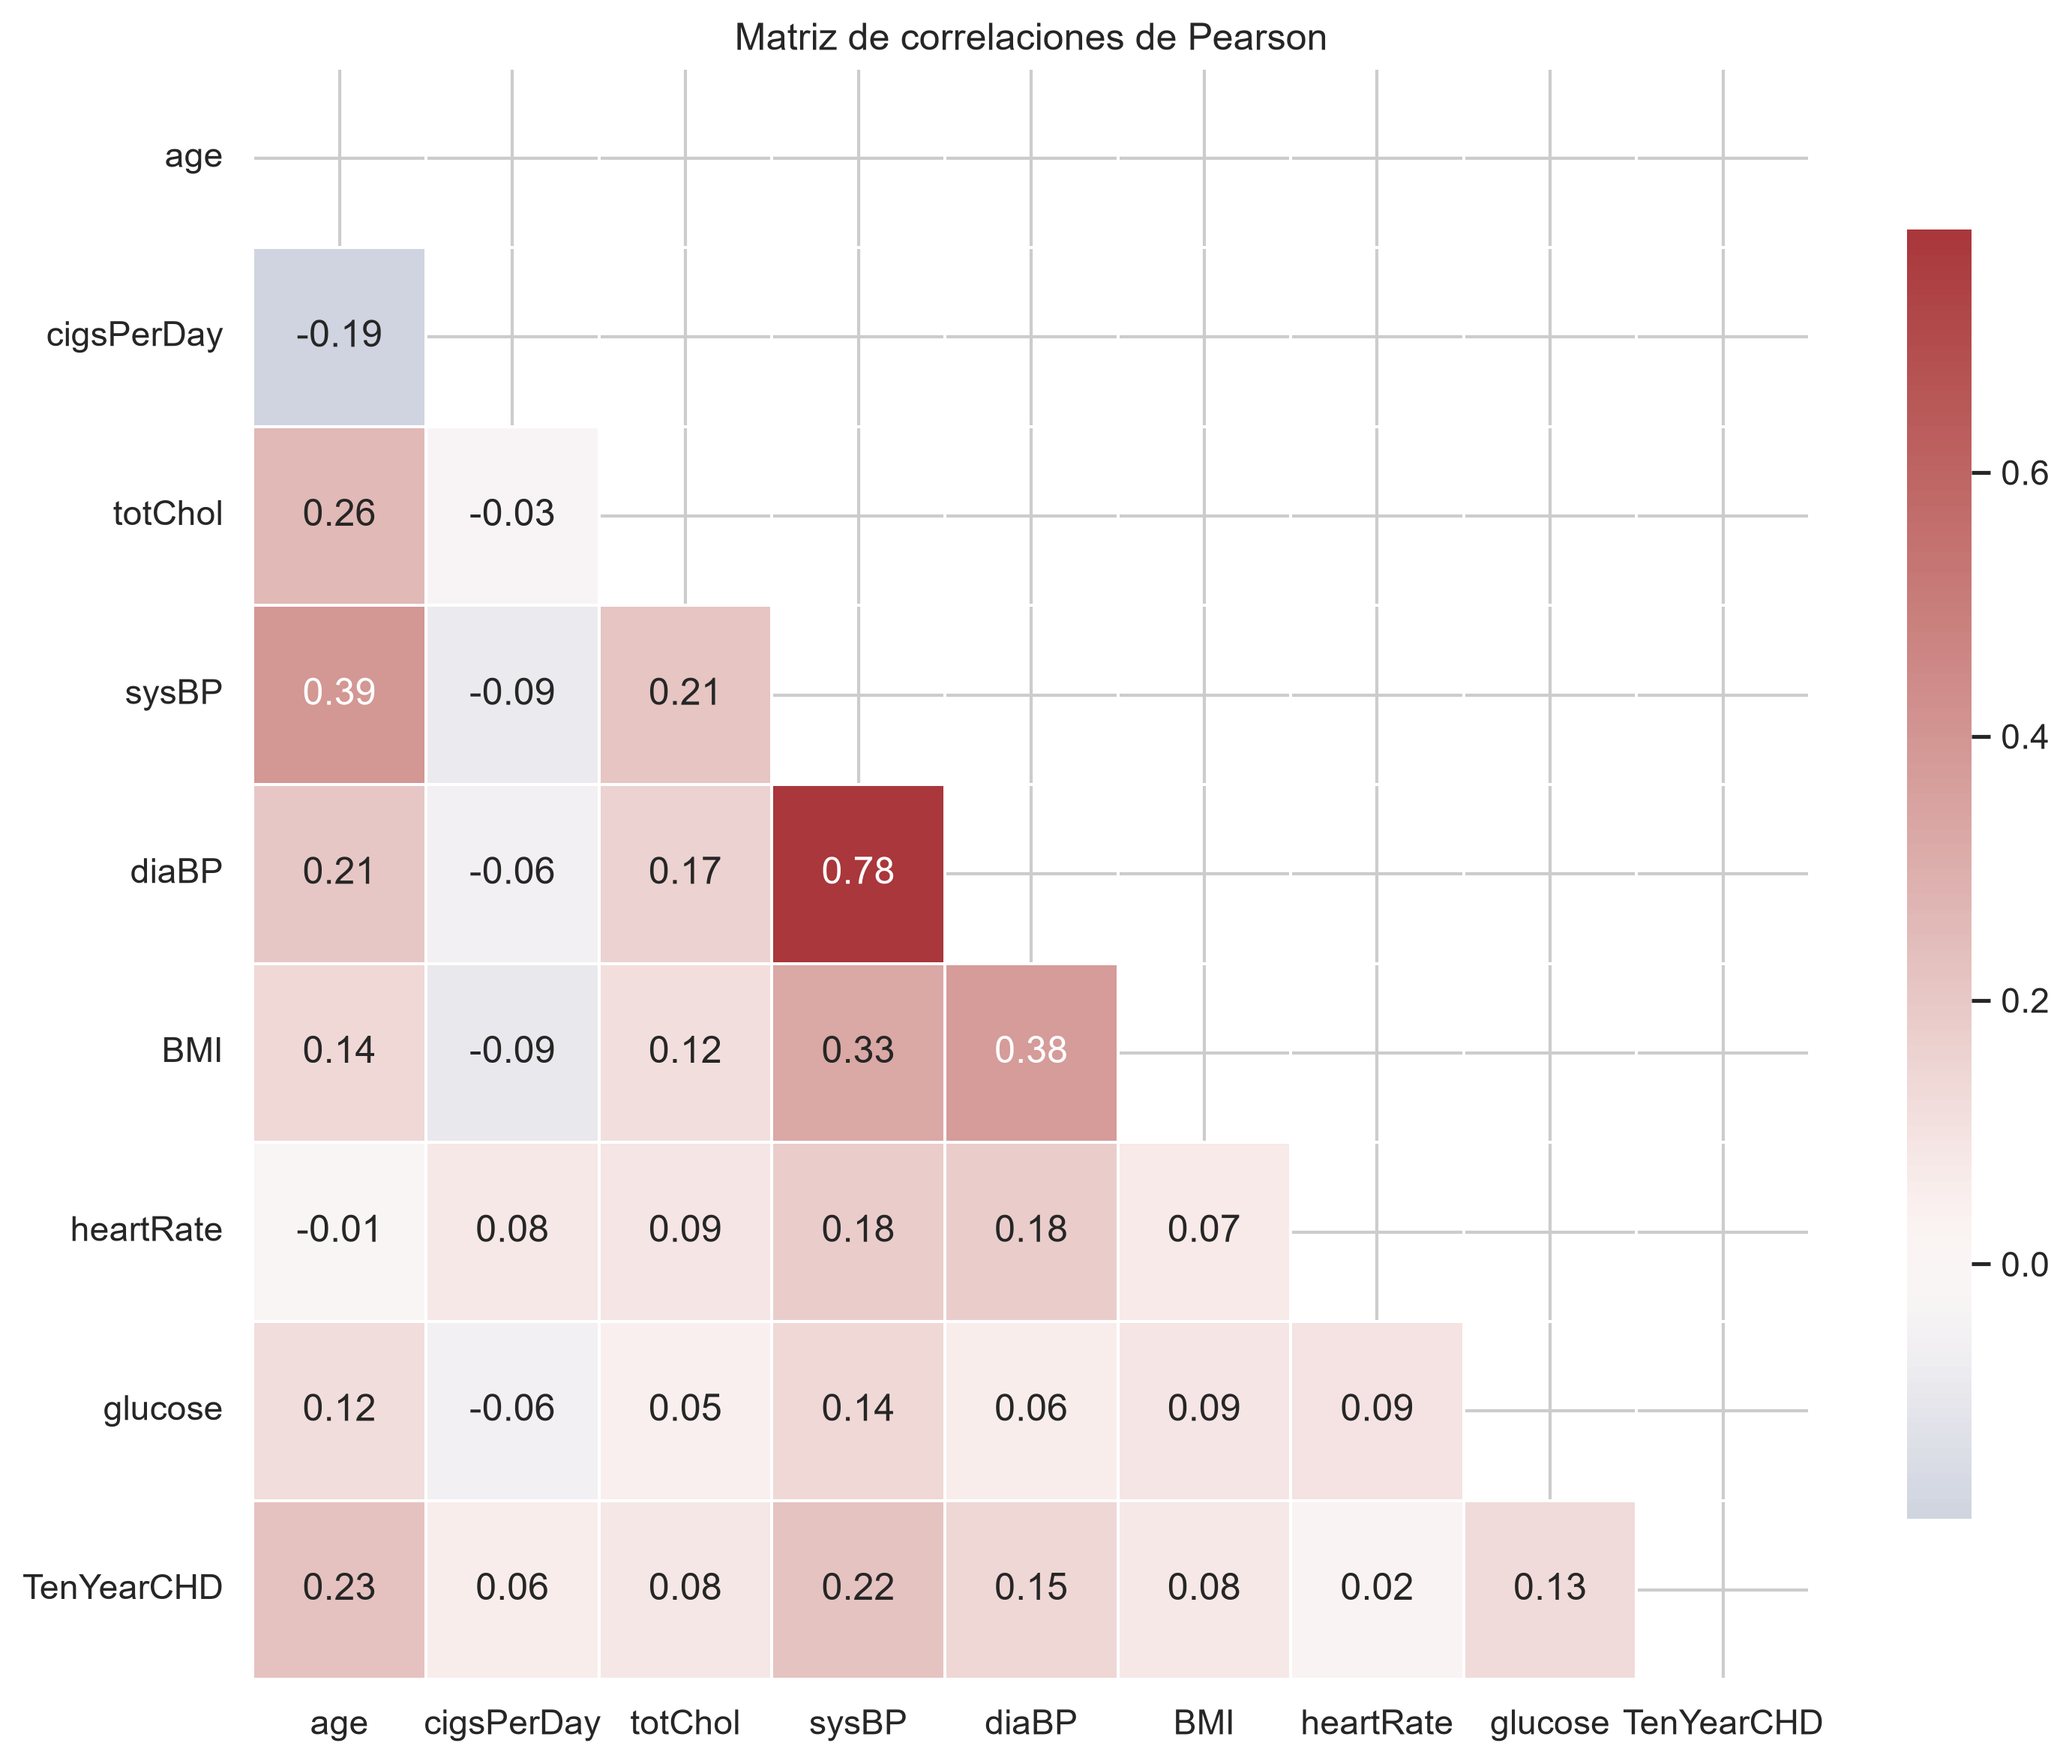
\includegraphics[width=0.61\textwidth]{../figuras/figura_3_correlaciones.png}
\caption{Matriz de correlaciones de Pearson (triángulo inferior).}
\label{fig:correlaciones}
\end{figure}

Los diagramas de caja muestran mayor edad y presión sistólica en el grupo con enfermedad. Para colesterol e IMC existe un solapamiento considerable, mientras glucosa contiene valores extremos. En el análisis categórico, 24,70\,\% de quienes presentan hipertensión desarrolló enfermedad, frente a 10,92\,\% del grupo sin dicho antecedente. En cambio, la diferencia descriptiva según tabaquismo actual es menor (15,9\,\% frente a 14,5\,\%) y debe interpretarse junto con intensidad, duración y edad.

% Guía oficial: tres variables numéricas, IC 95 %, justificación e interpretación.
\section{Estimación de parámetros}

Se estimaron las medias de edad, presión sistólica y colesterol total. Como la desviación estándar poblacional es desconocida, se utilizó un intervalo bilateral basado en $t$ de Student:
\[
\bar{x}\pm t_{0,975;n-1}\frac{s}{\sqrt{n}}.
\]
Los tamaños muestrales son grandes, pero el uso de $t$ mantiene explícita la incertidumbre asociada con la estimación de $s$. La Tabla~\ref{tab:intervalos} presenta los resultados.

\begin{table}[H]
\centering
\caption{Estimaciones puntuales e intervalos de confianza del 95\,\%.}
\label{tab:intervalos}
\small
\begin{tabular}{lrrr}
\toprule
\textbf{Parámetro} & \textbf{$n$} & \textbf{Estimación} & \textbf{IC 95\,\%} \\
\midrule
Edad media & 4.238 & 49,58 años & 49,33--49,84 \\
Presión sistólica media & 4.238 & 132,35 mmHg & 131,69--133,02 \\
Colesterol total medio & 4.188 & 236,72 mg/dL & 235,37--238,07 \\
Proporción de enfermedad coronaria & 4.238 & 15,20\,\% & 14,15\,\%--16,31\,\% \\
\bottomrule
\end{tabular}
\end{table}

Para la proporción se empleó el intervalo de Wilson, más estable que la aproximación normal simple para respuestas binarias. Los intervalos expresan rangos plausibles para parámetros poblacionales bajo los supuestos del muestreo; no contienen al 95\,\% de las observaciones individuales ni garantizan representatividad fuera de la población estudiada.

% Guía oficial: dos pruebas, H0/H1, alfa, supuestos, ejecución e implicancias.
\section{Pruebas de hipótesis}

Se fijó $\alpha=0,05$ antes de realizar dos contrastes bilaterales. La significancia se complementó con intervalos y tamaños de efecto.

\subsection{Presión sistólica según enfermedad coronaria}

Se planteó $H_0:\mu_{\mathrm{CHD}}=\mu_{\mathrm{sin\ CHD}}$ frente a $H_1:\mu_{\mathrm{CHD}}\neq\mu_{\mathrm{sin\ CHD}}$. Los grupos son independientes y numerosos; sus desviaciones difieren (26,69 frente a 20,46 mmHg), por lo que se aplicó $t$ de Welch. La media fue 143,62 mmHg con enfermedad ($n=644$) y 130,33 mmHg sin enfermedad ($n=3.594$). La diferencia fue 13,29 mmHg, IC 95\,\% $[11,11;15,46]$, con $t=12,015$, $gl=783,9$ y $p<0,001$. Se rechazó $H_0$. El tamaño $d=0,617$ indica una diferencia estandarizada moderada.

\subsection{Hipertensión previa y enfermedad coronaria}

Se contrastó $H_0$: ambas variables son independientes, frente a $H_1$: existe asociación. Todas las frecuencias esperadas superaron 199, por lo que se cumple el supuesto de chi-cuadrado. El resultado fue $\chi^2(1)=132,611$, $p<0,001$; se rechazó $H_0$. La magnitud fue baja a moderada ($V$ de Cramér $=0,177$). El riesgo observado fue 24,70\,\% con hipertensión y 10,92\,\% sin hipertensión, con riesgo relativo 2,26 y \textit{odds ratio} 2,68.

\begin{figure}[H]
\centering
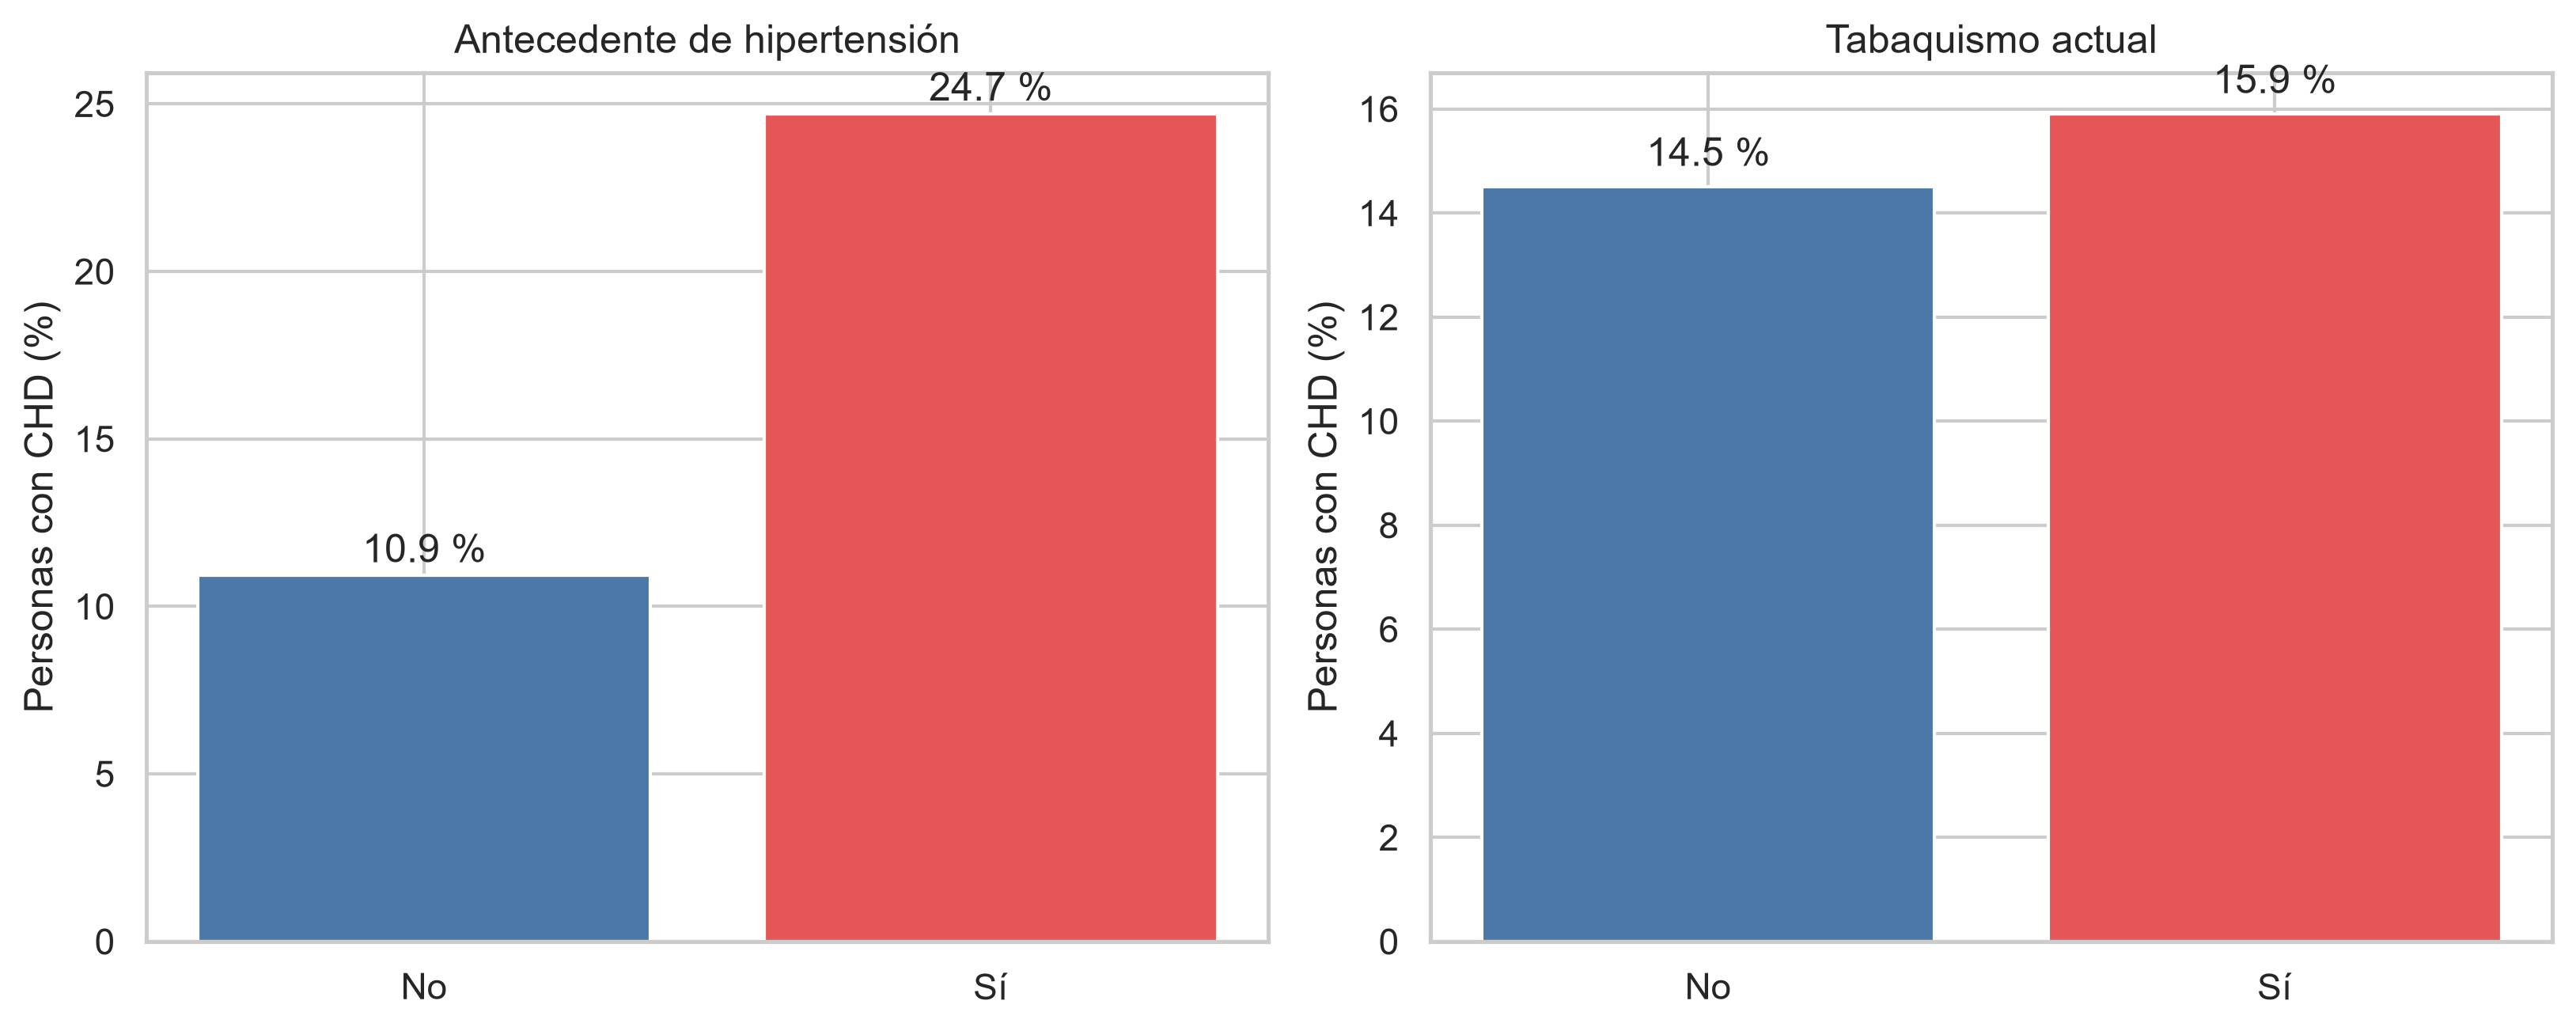
\includegraphics[width=0.70\textwidth]{../figuras/figura_5_tasas_categoricas.png}
\caption{Porcentaje de enfermedad coronaria según hipertensión y tabaquismo actual.}
\label{fig:tasas}
\end{figure}

Ambas pruebas describen asociaciones no ajustadas. No demuestran que presión sistólica o hipertensión causen por sí solas la enfermedad, pues edad, sexo, diabetes, tabaquismo y otros factores pueden confundir las comparaciones.

% Guía oficial: introducción, métodos, resultados, interpretación y próximos pasos.
\section{Informe de avance del proyecto}

El avance consolida un flujo reproducible desde datos crudos hasta evidencia descriptiva e inferencial. Los resultados destacan edad, presión arterial y antecedente de hipertensión como variables relevantes para profundizar el estudio cardiovascular. La incertidumbre se comunicó mediante intervalos y las decisiones inferenciales se acompañaron con tamaños de efecto.

Las limitaciones principales son el diseño observacional, el desbalance de la respuesta, los datos ausentes ---especialmente 9,16\,\% en glucosa--- y la ausencia de ajuste simultáneo por factores de confusión. Como próximos pasos se propone evaluar mecanismos de ausencia, definir un tratamiento reproducible de faltantes, estudiar relaciones multivariadas y comparar modelos predictivos con validación adecuada. Se mantendrá la distinción entre descripción, asociación, predicción y causalidad.

% Guía oficial: notebook reproducible y repositorio enlazado.
\section{Notebook y repositorio GitHub}

El notebook \path{fase-2/sumativa-1/notebooks/sumativa_1_framingham.ipynb} ejecuta 18 celdas de código sin errores, fija la semilla 42, localiza la raíz del proyecto, valida dimensiones y codificaciones y exporta cinco figuras a 300 dpi. Los datos originales permanecen en \path{fase-1/datos/raw/}; las dependencias están declaradas en \path{requirements.txt}. El historial y los entregables se encuentran en \proyRepo.

% Guía oficial: referencias APA 7 citadas explícitamente.
\begin{thebibliography}{9}
\raggedright

\bibitem{dileep}
Dileep, A. (2019). \textit{Logistic regression to predict heart disease} [Conjunto de datos]. Kaggle. \url{https://www.kaggle.com/datasets/dileep070/heart-disease-prediction-using-logistic-regression}

\bibitem{nhlbi}
National Heart, Lung, and Blood Institute. (s. f.). \textit{Teaching datasets: Framingham Heart Study}. \url{https://biolincc.nhlbi.nih.gov/teaching/}

\bibitem{scipy}
Virtanen, P., et al. (2020). SciPy 1.0: Fundamental algorithms for scientific computing in Python. \textit{Nature Methods, 17}, 261--272. \url{https://doi.org/10.1038/s41592-019-0686-2}

\bibitem{statsmodels}
Seabold, S., \& Perktold, J. (2010). Statsmodels: Econometric and statistical modeling with Python. En \textit{Proceedings of the 9th Python in Science Conference} (pp. 92--96). \url{https://doi.org/10.25080/Majora-92bf1922-011}

\end{thebibliography}

\end{document}
